\documentclass[aspectratio=169]{beamer}

% ---------- THEME & LOOK ----------
\usetheme{Madrid}
\usecolortheme{seahorse}
\usefonttheme{professionalfonts}
\setbeamertemplate{navigation symbols}{}
\setbeamercovered{transparent}
\setbeamertemplate{itemize items}[circle]
\setbeamertemplate{enumerate items}[default]
\setlength{\parskip}{0.25em}

% ---------- COLORS ----------
\usepackage{xcolor}
\definecolor{accent}{RGB}{0,92,184}
\definecolor{soft}{RGB}{233,244,255}
\setbeamercolor{structure}{fg=accent}
\setbeamercolor{title}{fg=white,bg=accent}
\setbeamercolor{frametitle}{fg=accent}
\setbeamercolor{block title}{bg=accent!10,fg=accent}
\setbeamercolor{block body}{bg=soft}

% ---------- PACKAGES ----------
\usepackage{booktabs}
\usepackage{amsmath, amssymb}
\usepackage{array}
\usepackage{graphicx}
\usepackage{hyperref}
\hypersetup{colorlinks=true,linkcolor=accent,urlcolor=accent}

% ---------- PLACEHOLDER BOX ----------
\newcommand{\placeholderbox}[2][0.82\linewidth]{%
  \begin{center}
    \fbox{\begin{minipage}[c][0.46\textheight][c]{#1}
      \centering \vspace{0.25em}
      \textbf{#2}\\[0.6em]
      \emph{Insert figure/table here later.}
    \end{minipage}}
  \end{center}
}

% ---------- TITLE ----------
\title{\textbf{The Economics of Immigration}}
\subtitle{{\large ECON 300 - Labour Economics}}
\author{Muhebullah Karimzada}
\date{Winter 2026}

\begin{document}

% ============================================================
% TITLE
% ============================================================
\begin{frame}[plain]
  \titlepage
\end{frame}

% ============================================================
\section{Orientation}
% ============================================================

\begin{frame}{Learning Objectives}
\transfade
\begin{itemize}
  \item Describe the profile of immigrants to Canada: how many arrive, where they come from, and where they settle.
  \item Explain Canada's point system and how it shapes immigrant selection.
  \item Use supply and demand to evaluate immigration's effects on wages and employment.
  \item Define \textbf{earnings assimilation} and explain why cross-section evidence can be misleading.
  \item Sketch a simple migration model and decision rule for moving countries.
\end{itemize}

\end{frame}

\begin{frame}{Main Questions}
\transfade
\begin{itemize}
  \item How have immigration patterns to Canada changed over the last 60 years?
  \item What is the point system, and how does it affect who immigrates?
  \item Do higher immigration inflows lower wages or raise unemployment?
  \item How quickly do immigrants' earnings catch up to native-born Canadians?
  \item Are immigrants a net fiscal burden or a net contribution?
\end{itemize}

\begin{exampleblock}{Example}
If a city receives many highly educated immigrants, the effects may differ from those of receiving many low-skilled immigrants. The impact depends on skills, occupations, and how labour demand adjusts.
\end{exampleblock}
\end{frame}

% ============================================================
\section{Immigration Patterns in Canada}
% ============================================================

\begin{frame}{Trends and Source Regions}
\transfade
\begin{itemize}
  \item Immigration levels fluctuated widely until the mid-1980s.
  \item Inflows were around 200,000 per year by the late 1990s and rose further after that.
  \item Per-capita inflows were high by international standards, though not always above Canada's own historical peaks.
  \item The regional origins of immigrants changed dramatically over time.
\end{itemize}

\begin{block}{Interpretation}
The size of immigration matters, but the \textbf{composition} of immigration matters just as much. Source-country changes can alter language profiles, education levels, labour market matching, and settlement patterns.
\end{block}
\end{frame}

\begin{frame}{Figure 11.1: Immigration to Canada by Source Region, 1955--2019}
\centering
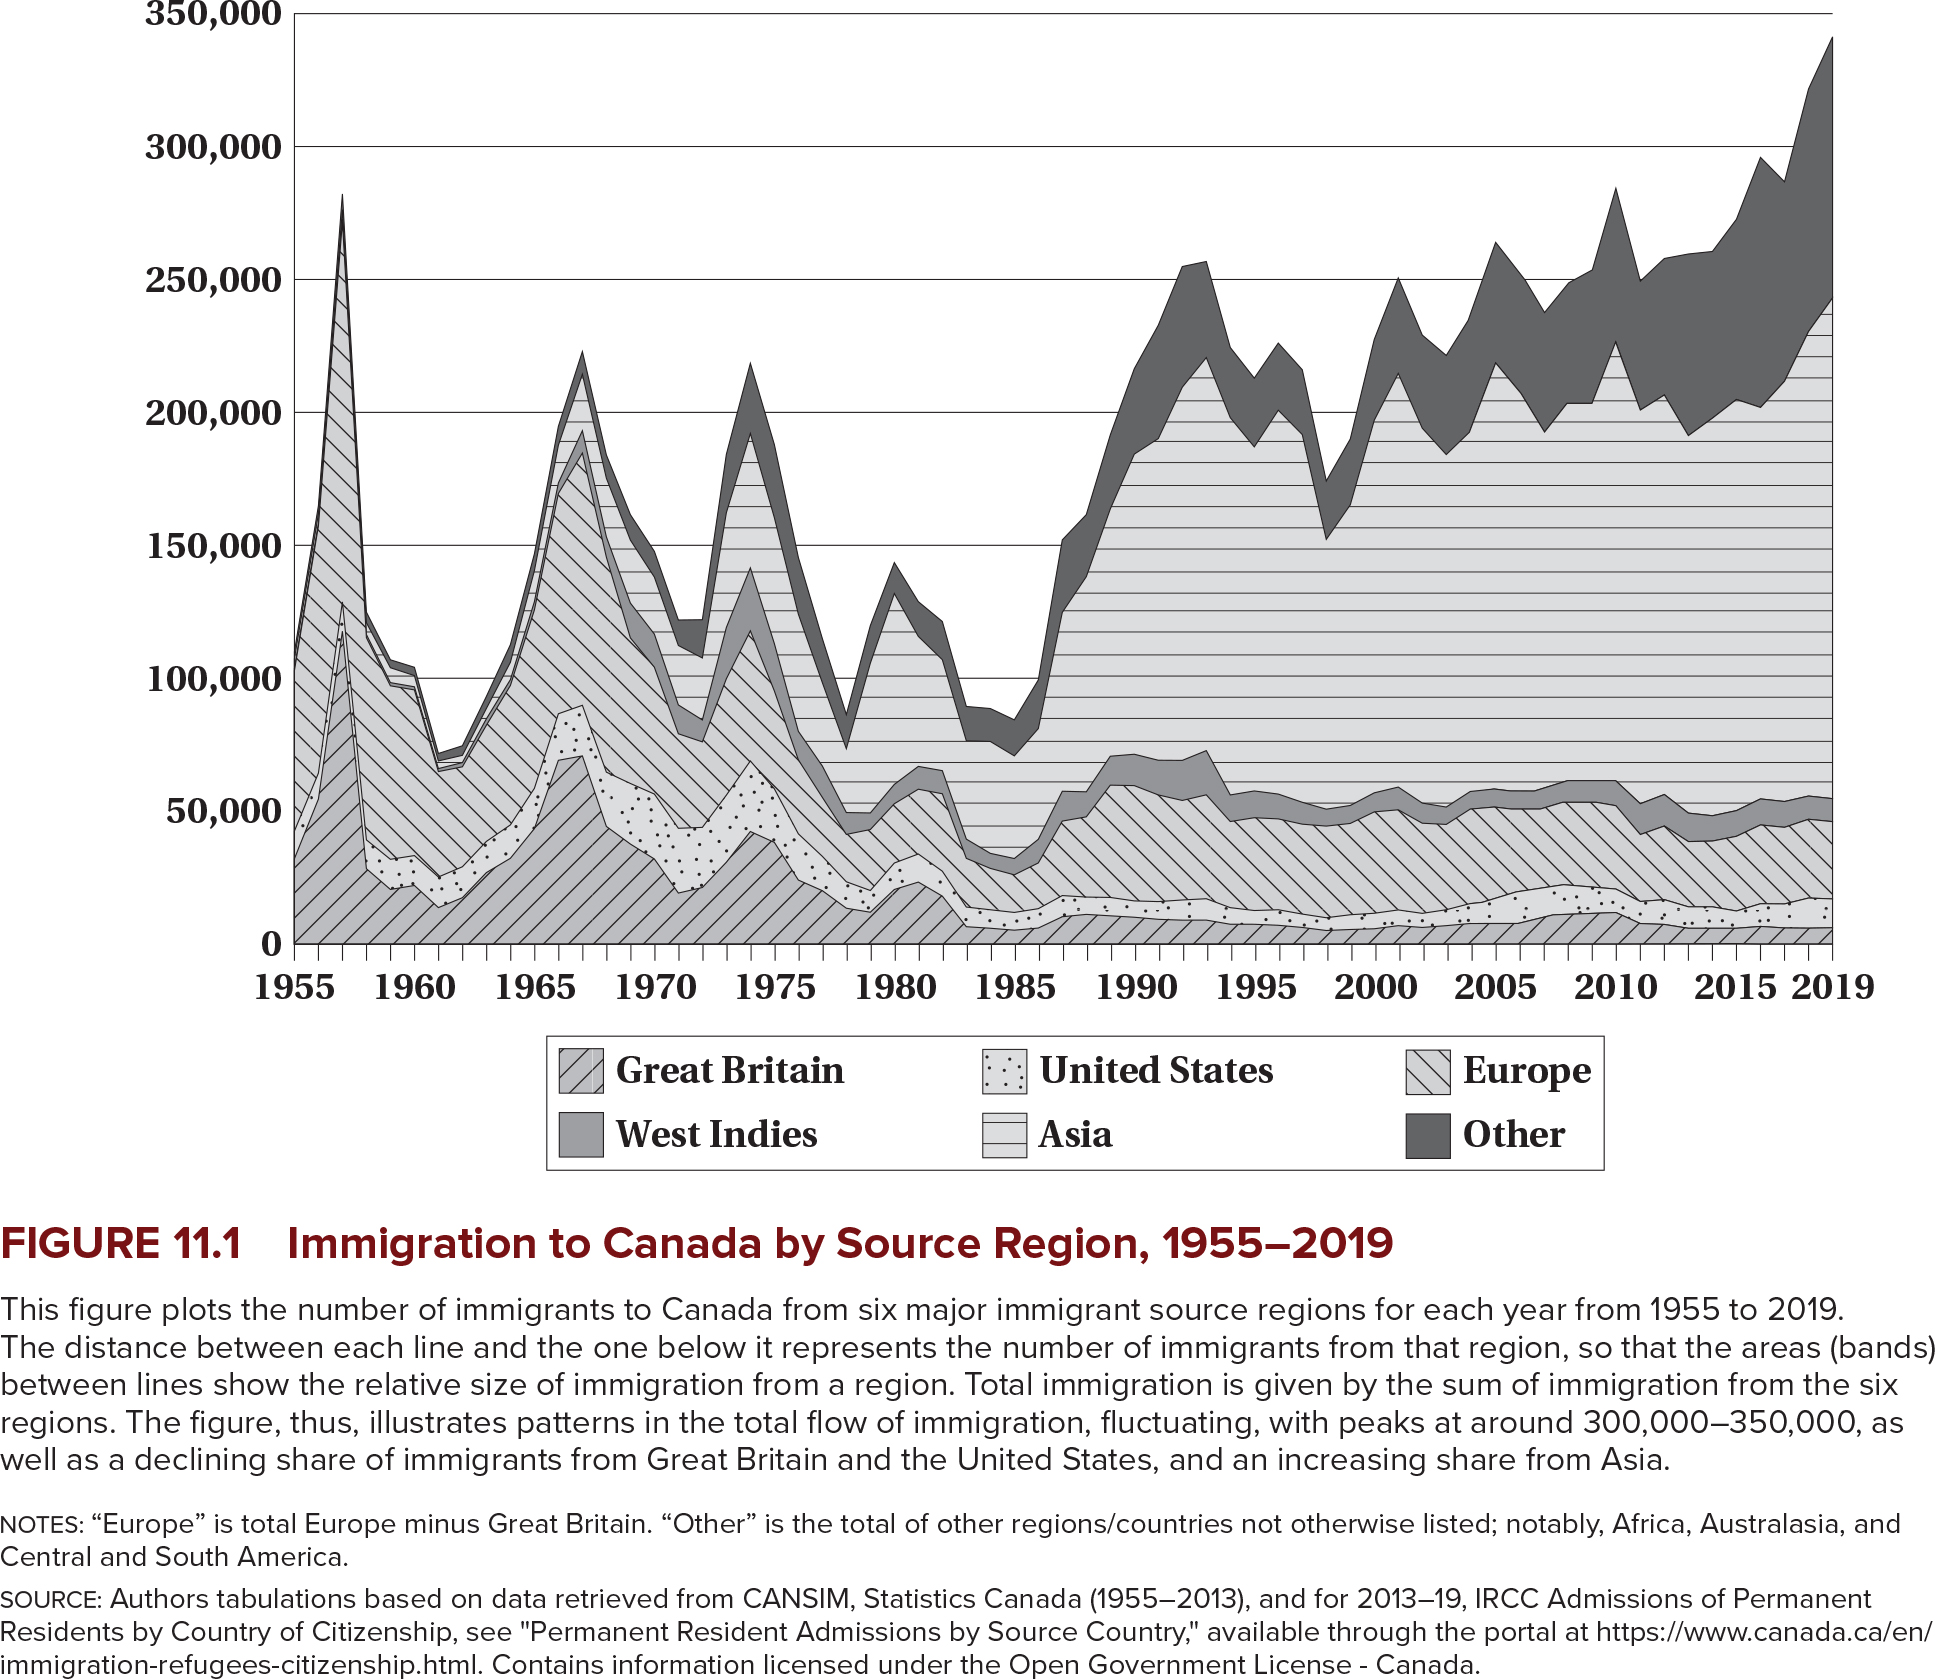
\includegraphics[width=0.8\linewidth]{ben54842_1101}
\end{frame}

\begin{frame}{Explaining Figure 11.1}
\transfade
\begin{itemize}
  \item Early postwar immigration was dominated by Europe, Great Britain, and the United States.
  \item Over time, Asia became the largest source region.
  \item Other regions also increased in importance, reflecting changes in Canadian immigration policy and global migration flows.
\end{itemize}

\begin{block}{Key Insight}
Canadian immigration shifted from a largely Europe-based flow to a much more globally diversified system.
\end{block}

\begin{exampleblock}{Example}
Changes in source regions can influence language acquisition, credential recognition, and the speed of labour market adjustment after arrival.
\end{exampleblock}
\end{frame}

\begin{frame}{Table 11.1: Top Ten Immigrant Source Countries, 2005 and 2019}
\centering
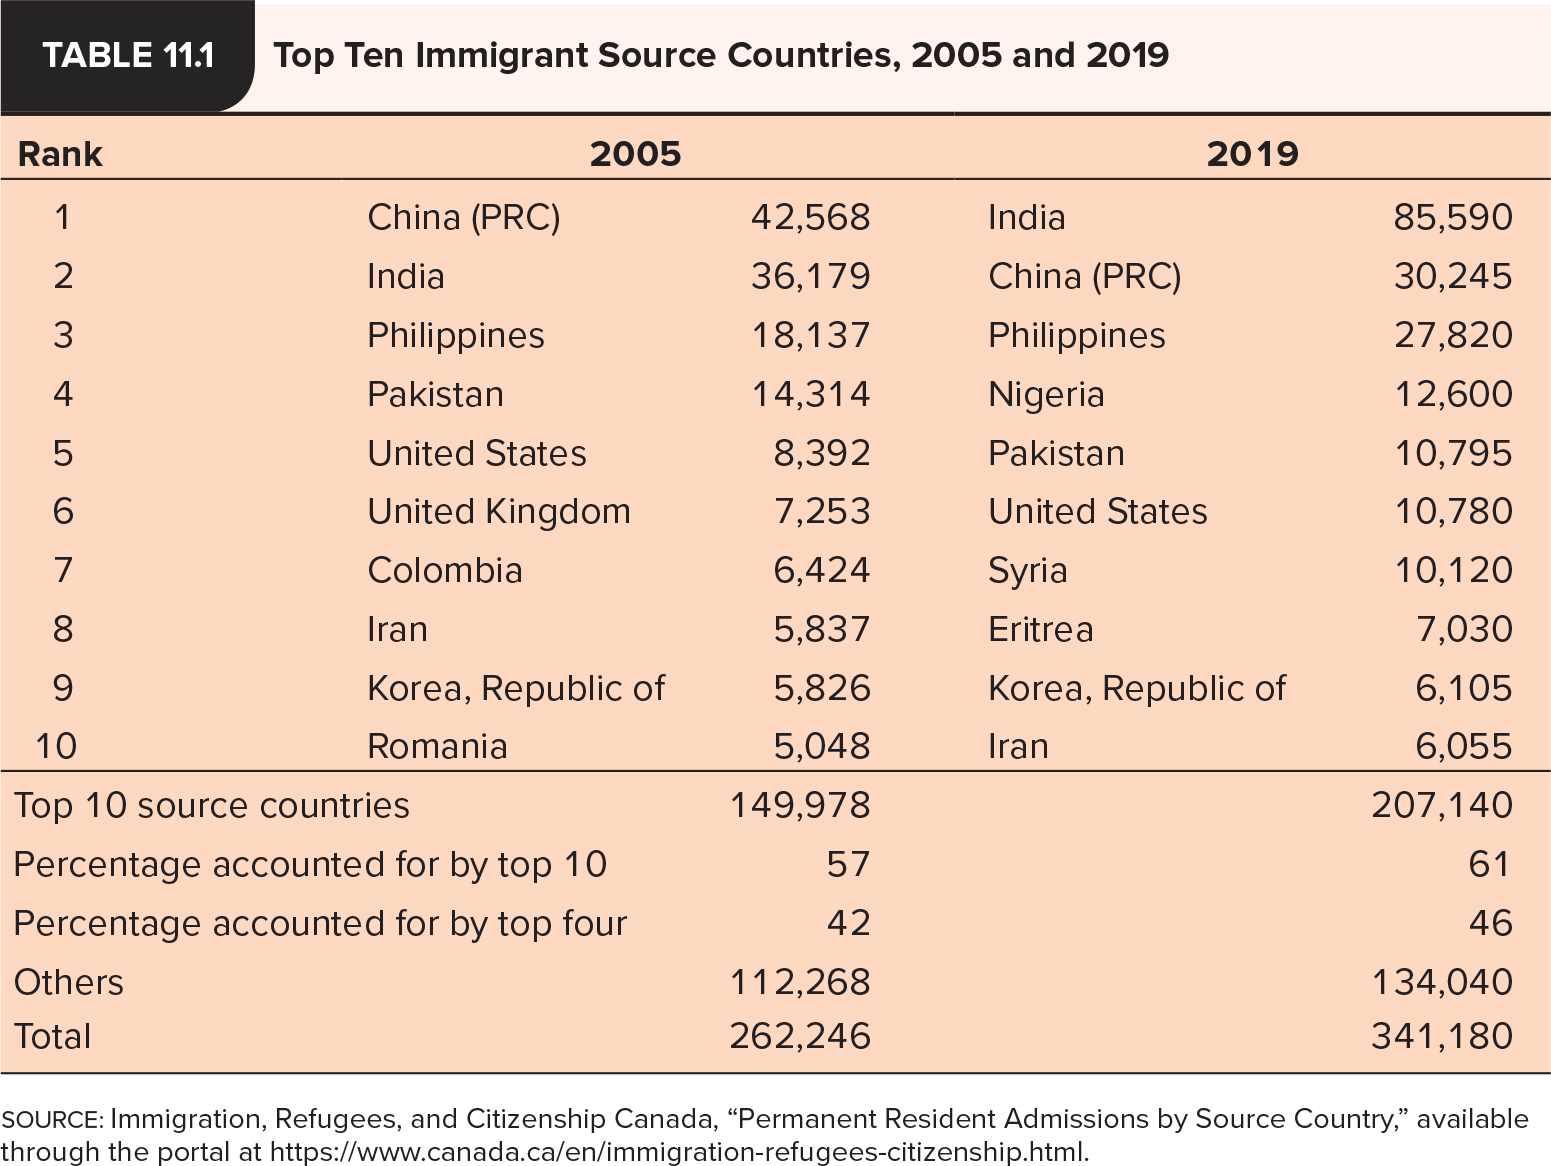
\includegraphics[width=0.64\linewidth]{ben54842_tb1101}
\end{frame}

\begin{frame}{Reading Table 11.1}
\transfade
\begin{itemize}
  \item The table lists the top source countries in 2005 and 2019.
  \item India and China are major source countries in both years.
  \item The concentration of immigrants among the top few source countries is substantial.
\end{itemize}

\begin{block}{Interpretation}
Source-country concentration matters because it can affect settlement networks, labour market matching, and demand for language and credential support services.
\end{block}
\end{frame}

\begin{frame}{Figure 11.2: Immigrant Concentration by CMA, 2006 and 2016}
\centering
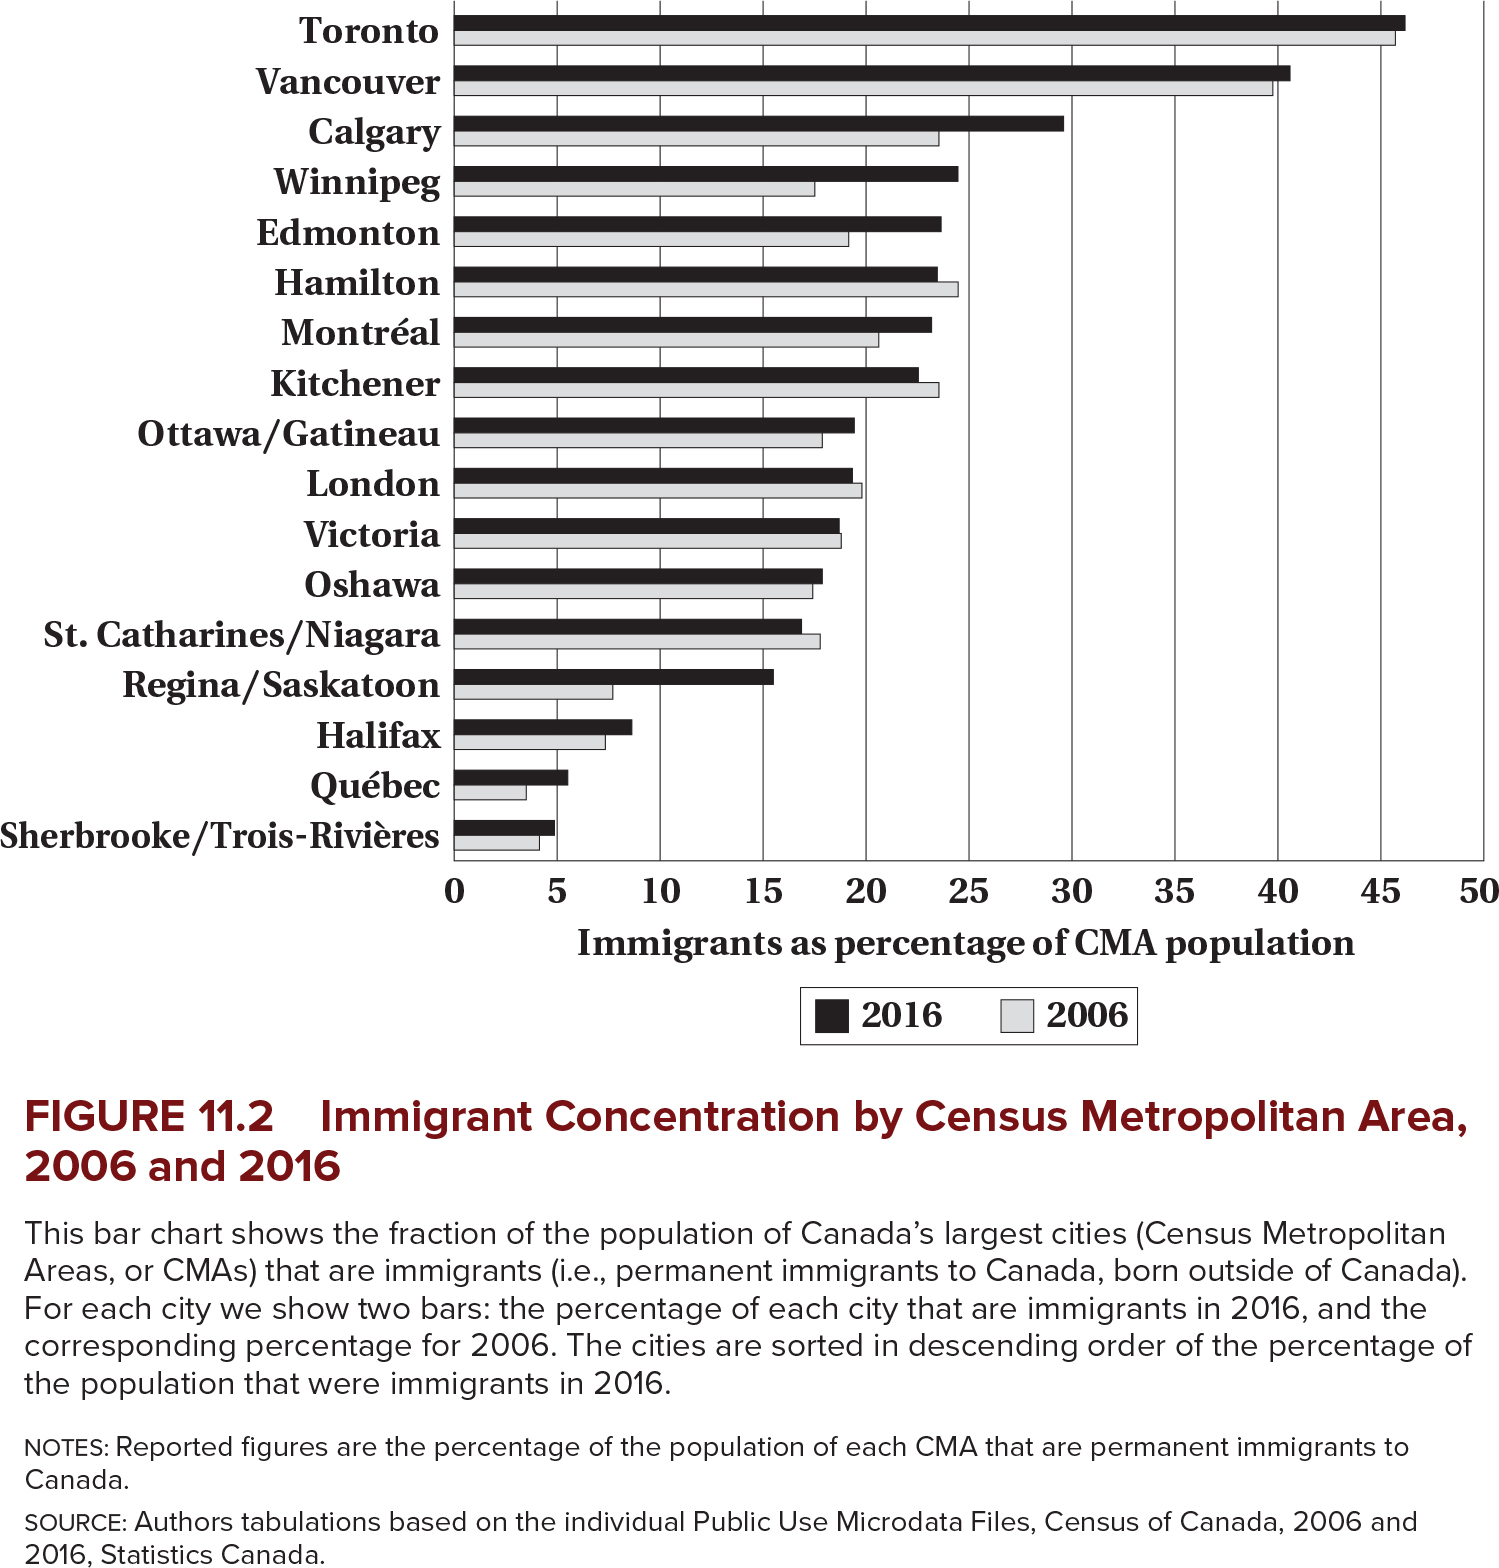
\includegraphics[width=0.7\linewidth]{ben54842_1102}
\end{frame}

\begin{frame}{Explaining Figure 11.2}
\transfade
\begin{itemize}
  \item Immigrants are heavily concentrated in a few major CMAs, especially Toronto and Vancouver.
  \item Some smaller CMAs have much lower immigrant shares.
  \item Concentration affects local labour markets, housing demand, and public services.
\end{itemize}

\begin{block}{Definition}
\textbf{CMA} means \textbf{Census Metropolitan Area}, a large urban labour market region used in Canadian statistics.
\end{block}

\begin{exampleblock}{Example}
A 5\% rise in immigrant share may have a different wage effect in Toronto than in a smaller city because of differences in industrial structure and housing constraints.
\end{exampleblock}
\end{frame}

% ============================================================
\section{Policy and Selection}
% ============================================================

\begin{frame}{Two Policy Levers}
\transfade
\begin{itemize}
  \item How many immigrants to admit.
  \item Who is admitted.
\end{itemize}

\begin{block}{Interpretation}
Immigration policy involves both \textbf{quantity} and \textbf{selection}. A country can change total admissions, change the mix of classes, or do both.
\end{block}
\end{frame}

\begin{frame}{Objectives of Immigration Policy}
\transfade
\begin{itemize}
  \item Maximize national welfare.
  \item Alleviate skill shortages and support economic growth.
  \item Promote family reunification.
  \item Provide humanitarian protection.
\end{itemize}

\begin{block}{Interpretation}
These goals do not always point in the same direction. For example, maximizing short-run labour market efficiency may conflict with humanitarian objectives.
\end{block}
\end{frame}

\begin{frame}{Two Admission Classes}
\transfade
\begin{itemize}
  \item \textbf{Assessed class:} independent immigrants evaluated on expected labour-market success.
  \item \textbf{Non-assessed class:} family and refugee classes.
\end{itemize}

\begin{block}{Definition}
\textbf{Assessed immigrants} are selected partly on expected economic performance, while \textbf{non-assessed immigrants} are admitted mainly through family reunification or humanitarian criteria.
\end{block}
\end{frame}

\begin{frame}{Canada's Immigration Point System (circa 2016)}
\transfade
\begin{itemize}
  \item At least one year of recent full-time experience in a broadly skilled occupation.
  \item Minimum score on an approved language test.
  \item Sufficient start-up funds on arrival.
  \item Minimum total score of 67 out of 100.
\end{itemize}

\begin{block}{Six Main Criteria}
\begin{itemize}
  \item Education (25)
  \item Official language (28)
  \item Work experience (15)
  \item Age (10)
  \item Arranged employment (10)
  \item Adaptability (10)
\end{itemize}
\end{block}
\end{frame}

\begin{frame}{Why a Point System?}
\transfade
\begin{itemize}
  \item It shifts selection toward workers expected to succeed in the labour market.
  \item It gives policymakers a flexible way to reweight desirable characteristics.
  \item It can improve average earnings outcomes of immigrants if the chosen criteria predict productivity.
\end{itemize}

\begin{exampleblock}{Example}
A higher weight on official language proficiency may improve immigrants' short-run labour market integration because communication skills matter in many occupations.
\end{exampleblock}
\end{frame}

\begin{frame}{Figure 11.3: Immigration to Canada by Class, 1966--2019}
\centering
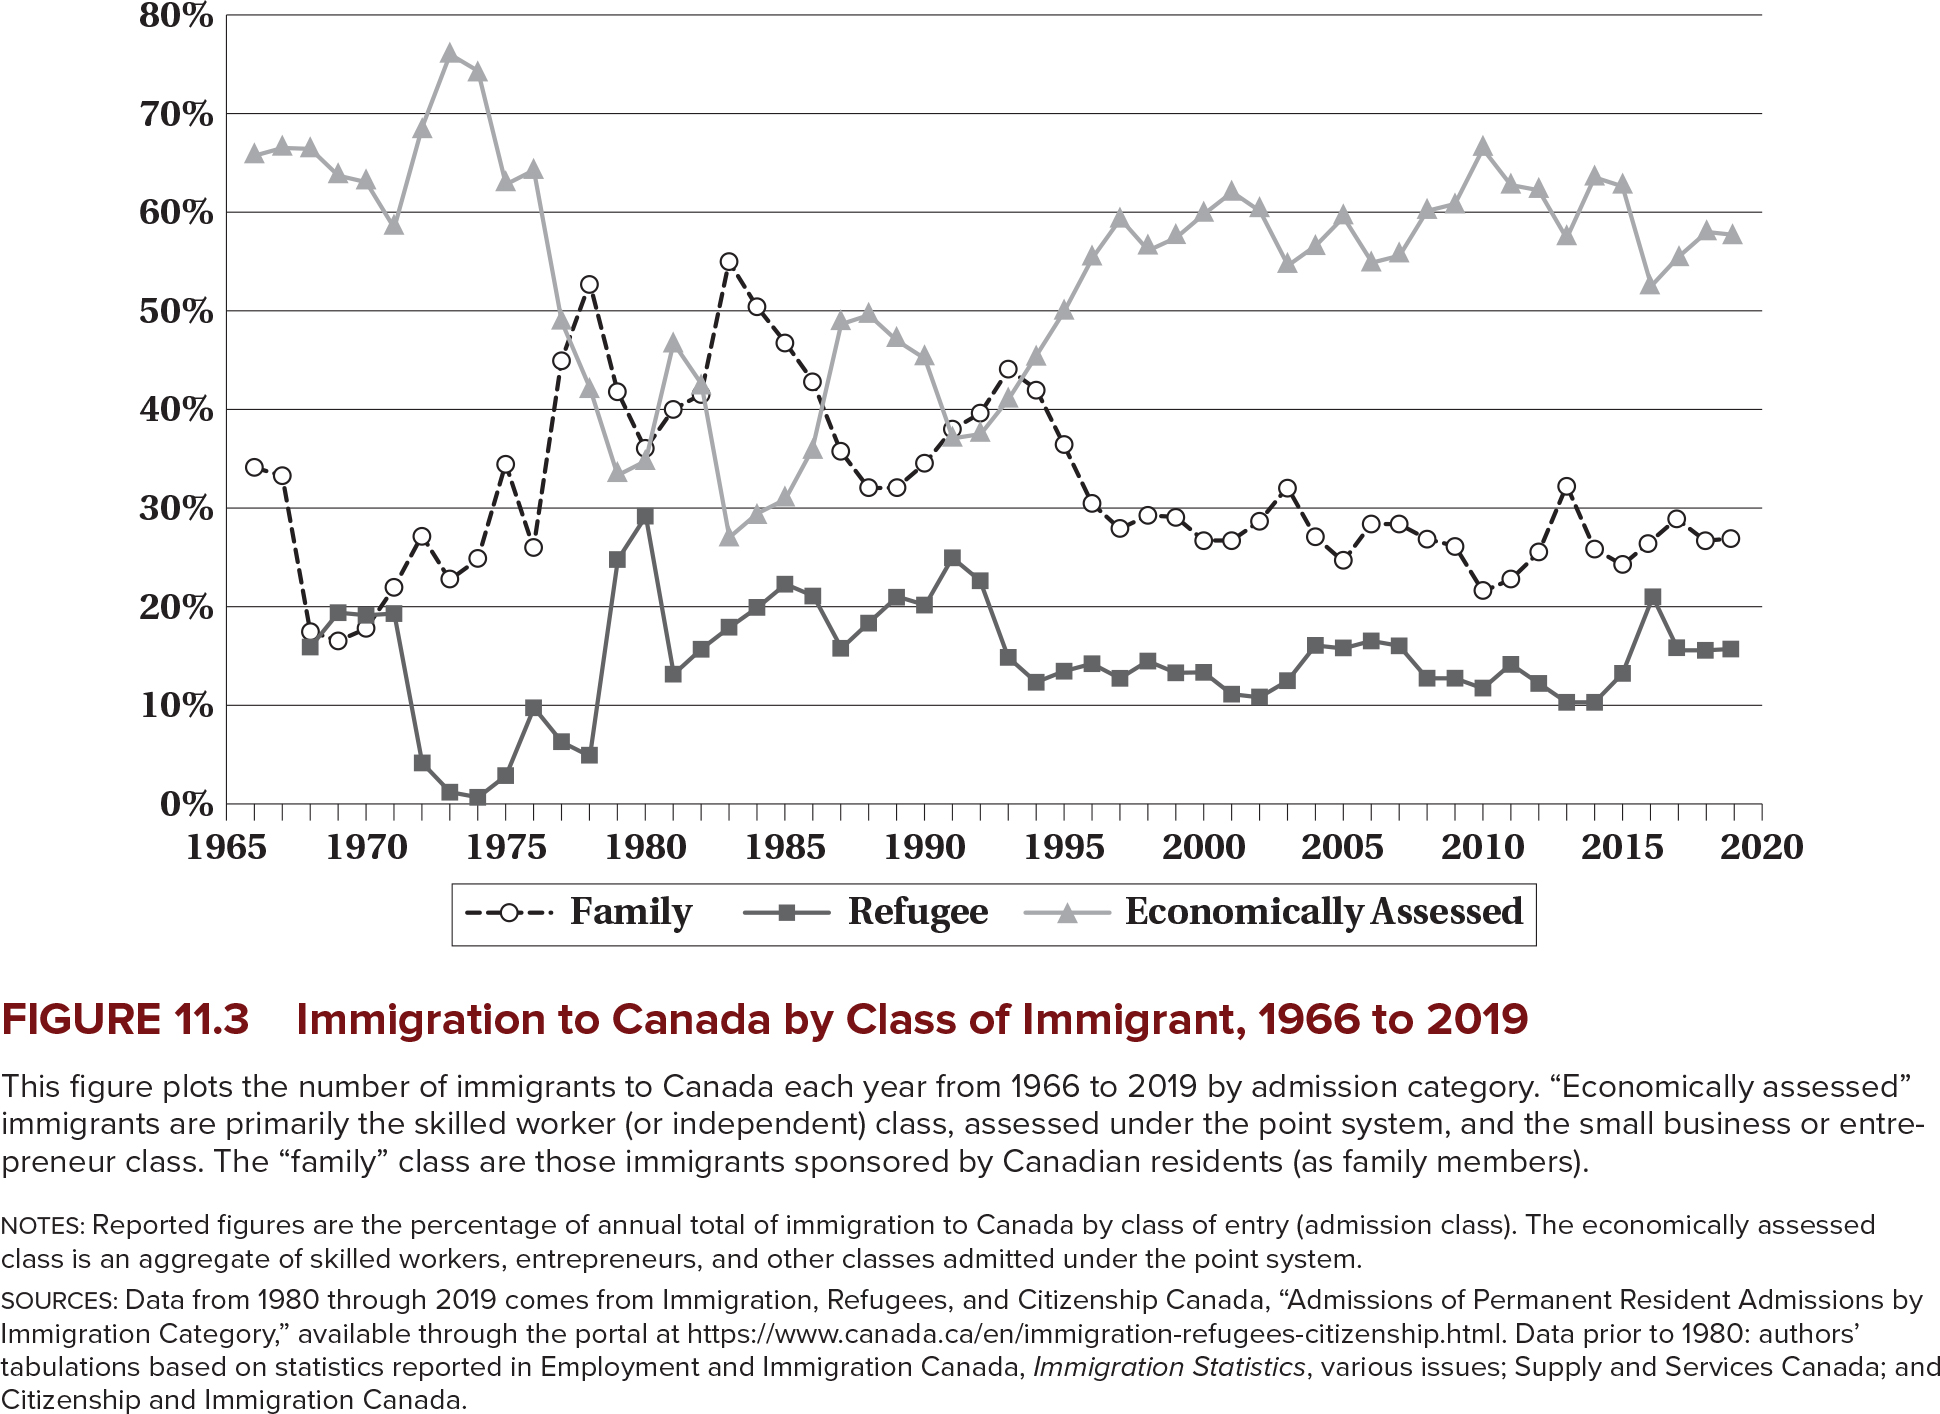
\includegraphics[width=0.96\linewidth]{ben54842_1103}
\end{frame}

\begin{frame}{Explaining Figure 11.3}
\transfade
\begin{itemize}
  \item The relative importance of family, refugee, and economically assessed immigrants changes over time.
  \item Economically assessed immigrants account for a large share in many years.
  \item Family and refugee categories remain important parts of total admissions.
\end{itemize}

\begin{block}{Interpretation}
Changes in class composition influence average labour market outcomes because assessed immigrants are selected more directly on expected labour market performance.
\end{block}
\end{frame}

% ============================================================
\section{Labour Market Effects}
% ============================================================

\begin{frame}{Supply--Demand Logic}
\transfade
\begin{itemize}
  \item Immigration shifts labour supply right in receiving markets.
  \item Wage and employment effects depend on:
  \begin{itemize}
    \item labour supply elasticity,
    \item labour demand elasticity,
    \item capital adjustment,
    \item the skill composition of immigrants.
  \end{itemize}
  \item Whether immigrants are substitutes or complements for native-born workers is crucial.
\end{itemize}
\end{frame}

\begin{frame}{Definition: Substitutes vs. Complements}
\transfade
\begin{block}{Substitutes}
Two groups are \textbf{substitutes} if an increase in one group's labour supply reduces the marginal productivity of the other.
\end{block}

\begin{block}{Complements}
Two groups are \textbf{complements} if an increase in one group's labour supply raises the marginal productivity of the other.
\end{block}

\begin{exampleblock}{Example}
High-skilled immigrants in engineering may complement local technicians and administrative staff, raising productivity for those groups.
\end{exampleblock}
\end{frame}

\begin{frame}{Figure 11.4: Impact of Immigration on Employment and Wages}
\centering
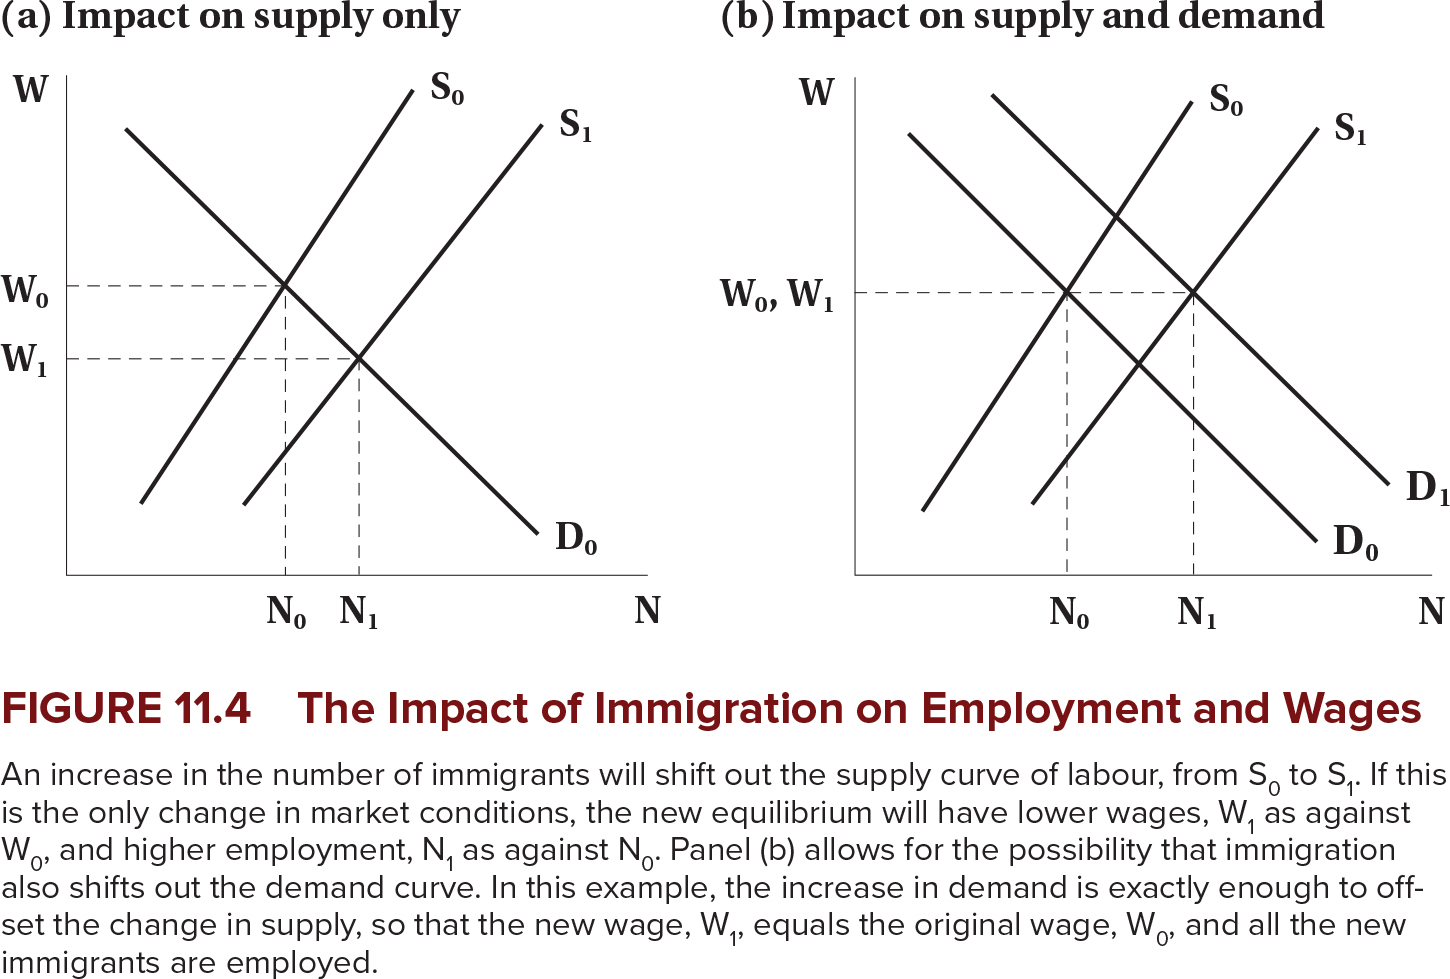
\includegraphics[width=0.72\linewidth]{ben54842_1104}
\end{frame}

\begin{frame}{Explaining Figure 11.4}
\transfade
\begin{itemize}
  \item Panel (a): if immigration shifts labour supply only, wages fall and employment rises.
  \item Panel (b): if immigration also raises labour demand, wage effects may be smaller or even negligible.
  \item Capital adjustment, consumption demand, and entrepreneurship can all shift labour demand.
\end{itemize}

\begin{block}{Interpretation}
The simple ``more workers means lower wages'' story may be too narrow because immigration can also expand demand and capital accumulation.
\end{block}
\end{frame}

\begin{frame}{Estimating the Effects: Strategies}
\transfade
\begin{itemize}
  \item \textbf{Counterfactual problem:} what would wages have been without immigration?
  \item \textbf{Cross-city variation:} compare high- and low-immigration cities.
  \item \textbf{Natural experiments:} exploit sudden inflow shocks.
  \item \textbf{Combined approaches:} improve identification by using multiple strategies.
\end{itemize}

\begin{block}{Definition}
A \textbf{natural experiment} is a situation where economic conditions create variation that resembles random assignment.
\end{block}
\end{frame}

\begin{frame}{Findings from Empirical Research}
\transfade
\begin{itemize}
  \item It is difficult to find strong adverse average effects on the native-born.
  \item Effects are highly skill-specific.
  \item Some groups may gain while others lose, depending on substitutability.
\end{itemize}

\begin{block}{Interpretation}
Average effects can hide important distributional effects across education, experience, and occupation groups.
\end{block}
\end{frame}

% ============================================================
\section{Assimilation}
% ============================================================

\begin{frame}{Assimilation Concepts}
\transfade
\begin{block}{Definition}
\textbf{Earnings assimilation} is the process by which immigrants' earnings move closer to those of comparable native-born workers over time in the host country.
\end{block}

\begin{itemize}
  \item Immigrants may begin with lower hours or earnings.
  \item Over time, earnings may rise because of:
  \begin{itemize}
    \item language acquisition,
    \item local work experience,
    \item credential recognition,
    \item job matching improvements.
  \end{itemize}
\end{itemize}
\end{frame}

\begin{frame}{Figure 11.5: Hypothetical Assimilation Profile}
\centering
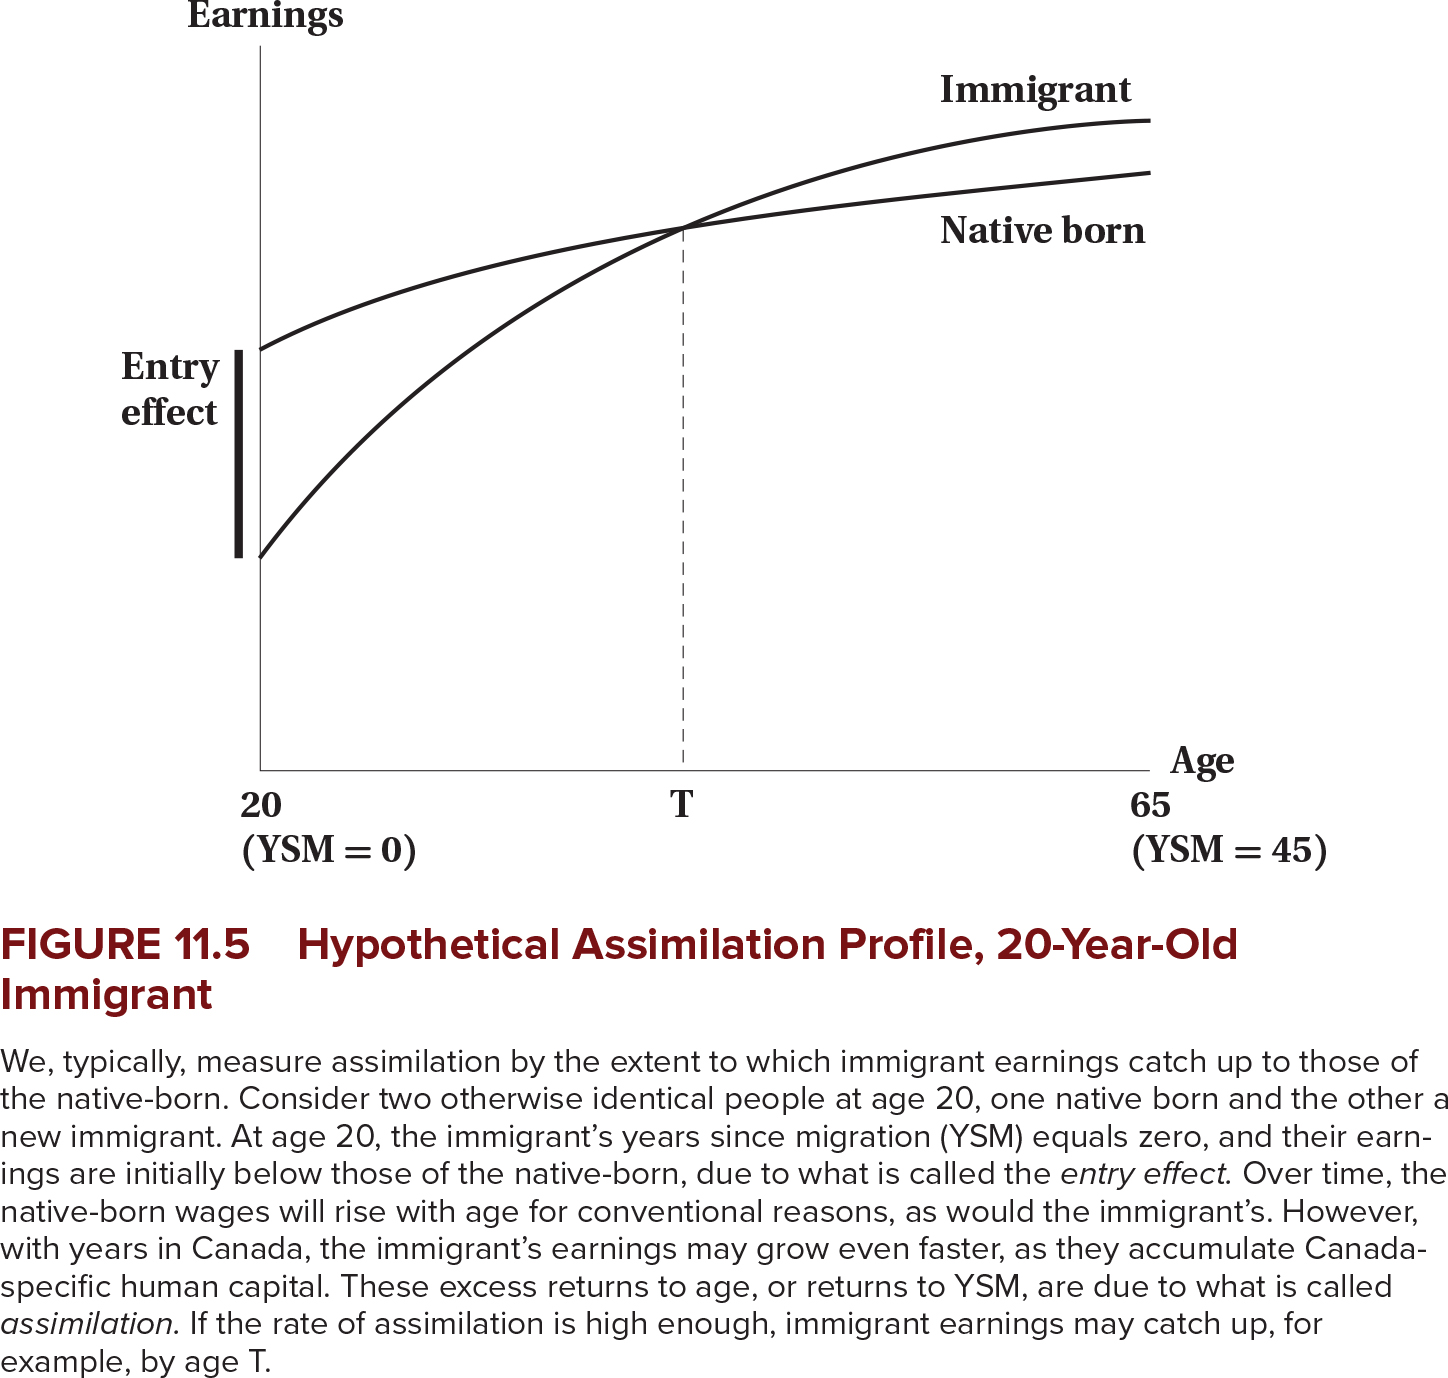
\includegraphics[width=0.8\linewidth]{ben54842_1105}
\end{frame}

\begin{frame}{Explaining Figure 11.5}
\transfade
\begin{itemize}
  \item The immigrant earnings profile starts below the native-born profile.
  \item The initial gap is the \textbf{entry effect}.
  \item Over time, immigrant earnings grow faster and may eventually approach or exceed native-born earnings.
\end{itemize}

\begin{block}{Interpretation}
Assimilation is about \textbf{growth after arrival}, not just about the initial earnings gap.
\end{block}
\end{frame}

\begin{frame}{Measuring Assimilation Properly}
\transfade
\begin{itemize}
  \item Cross-sections mix together:
  \begin{itemize}
    \item time since arrival,
    \item cohort quality,
    \item macroeconomic conditions.
  \end{itemize}
  \item Quasi-panels track cohorts over time and separate assimilation from cohort effects.
\end{itemize}

\begin{block}{Definition}
A \textbf{cohort effect} is a difference across arrival groups, not a change within the same immigrant group over time.
\end{block}
\end{frame}

\begin{frame}{Figure 11.6: Disentangling Cohort vs. Assimilation Effects}
\centering
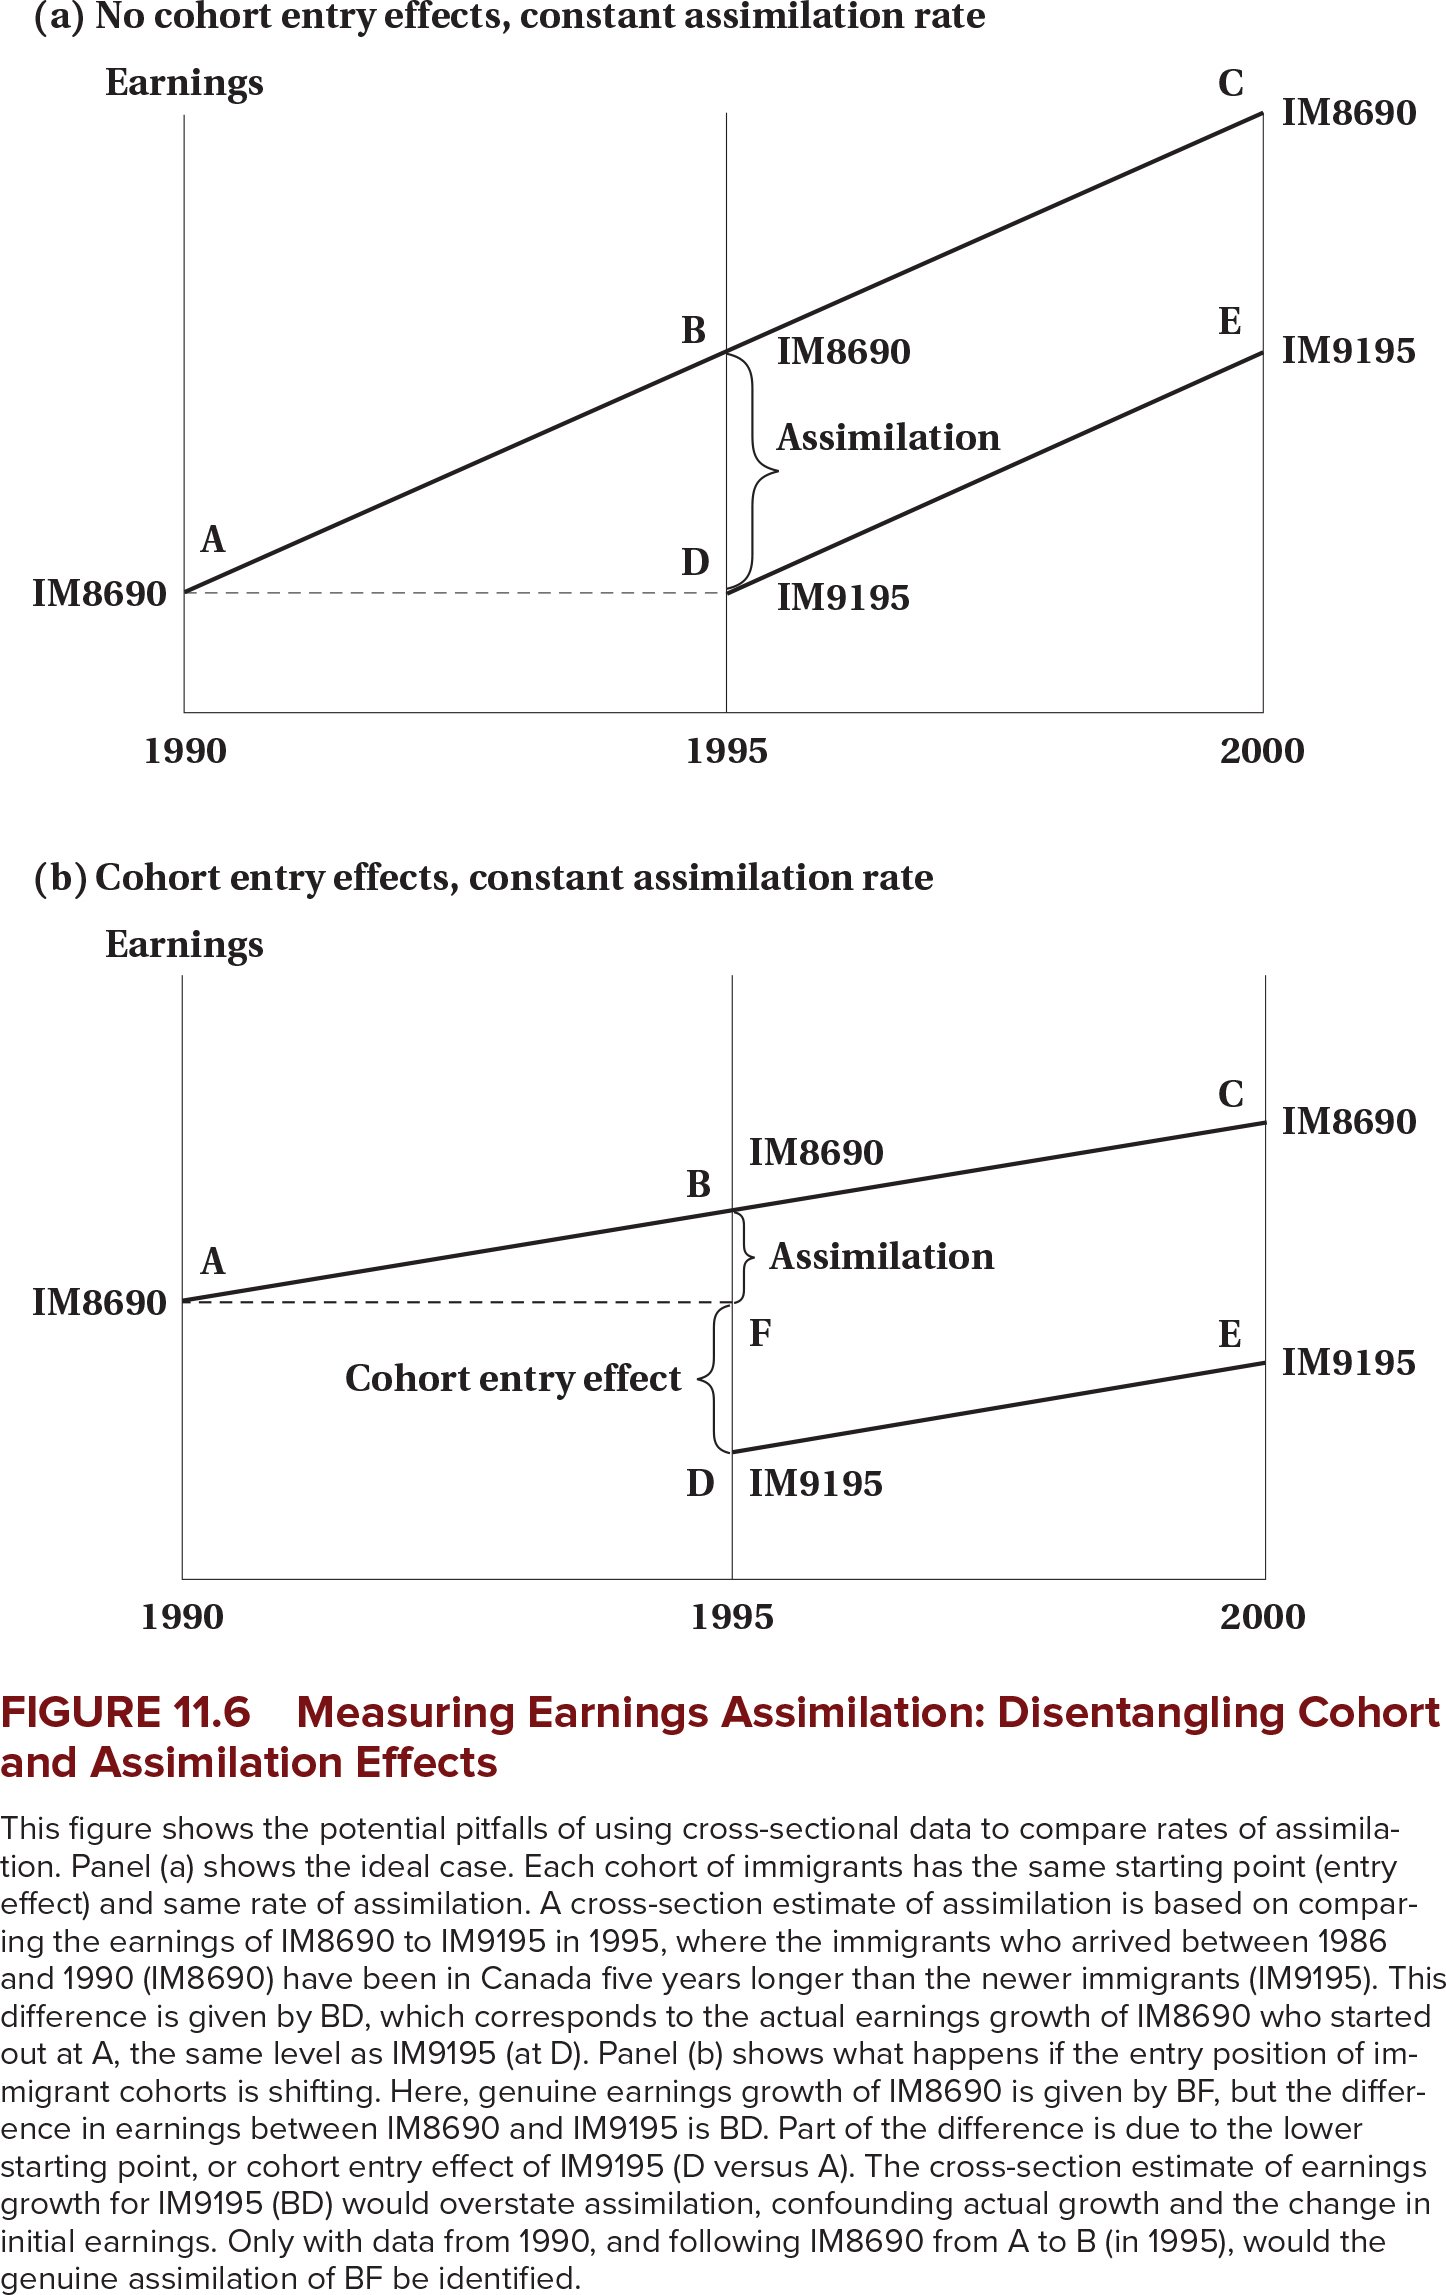
\includegraphics[width=0.425\linewidth]{ben54842_1106}
\end{frame}

\begin{frame}{Reading Figure 11.6}
\transfade
\begin{itemize}
  \item Panel (a): if cohort quality is constant, observed wage growth reflects assimilation.
  \item Panel (b): if cohort quality worsens over time, cross-section comparisons overstate assimilation.
  \item A newer, weaker cohort can make earlier cohorts look like they assimilate faster than they actually do.
\end{itemize}

\begin{block}{Key Point}
Cross-sections can confound \textbf{who arrived} with \textbf{how much they improved}.
\end{block}
\end{frame}

\begin{frame}{Figure 11.7: Annual Earnings by Immigrant Cohort, 2010 and 2015}
\centering
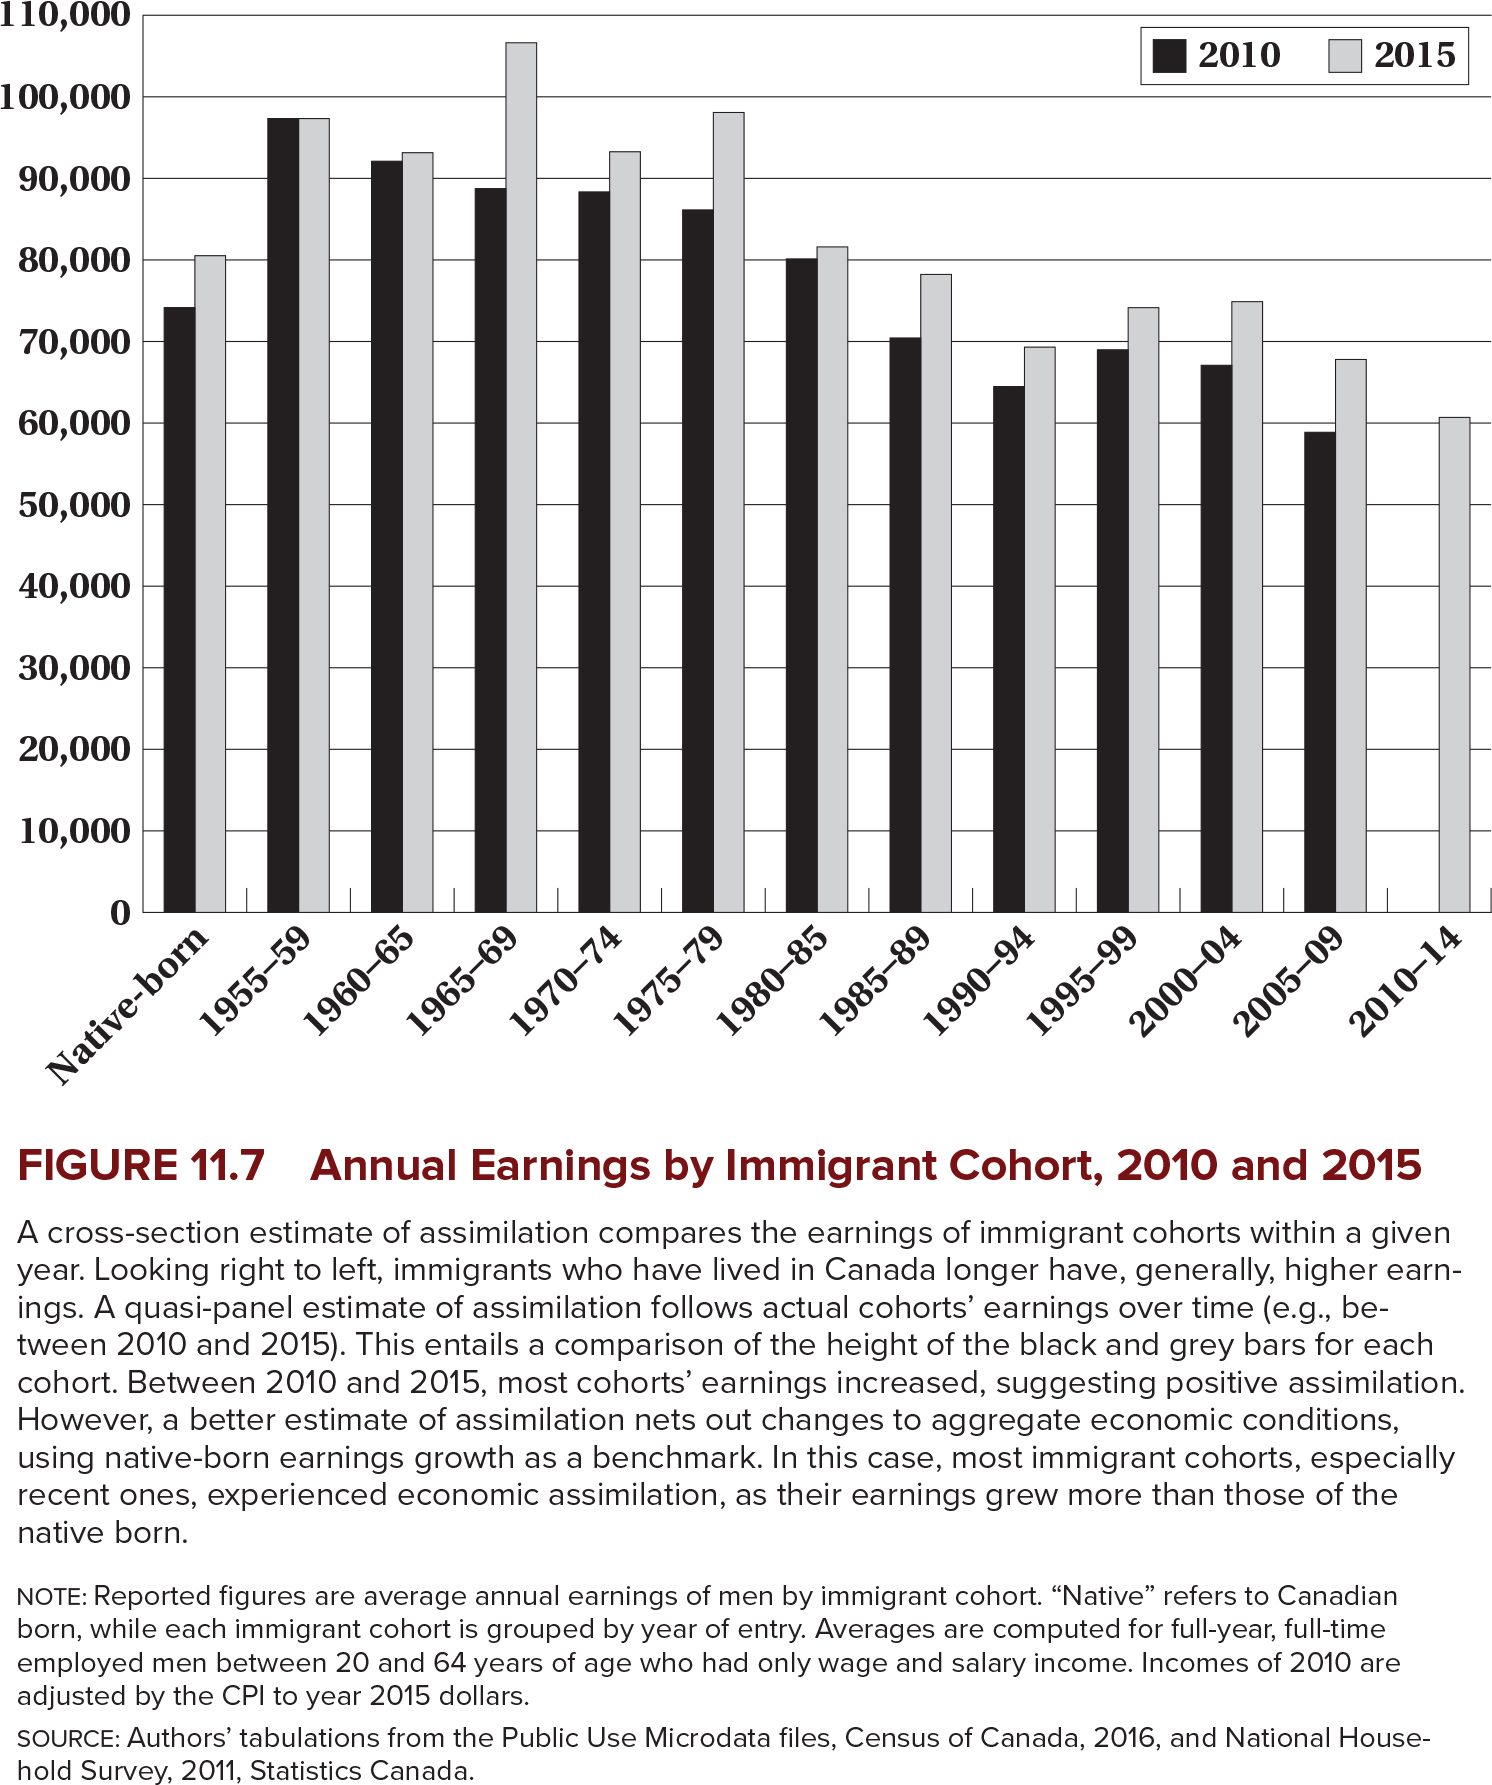
\includegraphics[width=0.67\linewidth]{ben54842_1107}
\end{frame}

\begin{frame}{Worked Example: Cross-Section vs. Quasi-Panel}
\transfade
Suppose the data report:

\begin{itemize}
  \item Native born: \$46,999 in 1995, \$48,641 in 2000
  \item IM9195 cohort: \$31,423 in 1995, \$38,652 in 2000
\end{itemize}

Then:
\[
\text{Entry effect} = 46{,}999 - 31{,}423 = 15{,}576
\]

Cross-section ``assimilation'':
\[
36{,}580 - 31{,}423 = 5{,}157
\]

Quasi-panel assimilation net of natives:
\[
7{,}229 - 1{,}642 = 5{,}587
\]

\begin{block}{Interpretation}
Tracking the same cohort over time gives a cleaner estimate of assimilation than simply comparing different cohorts in one year.
\end{block}
\end{frame}

\begin{frame}{Empirical Evidence on Assimilation}
\transfade
\begin{itemize}
  \item Entry penalties have generally worsened over time.
  \item Returns to foreign education and experience are often lower than returns to Canadian-acquired credentials.
  \item Many cohorts do not fully catch up to native-born earnings on average.
  \item Women often show somewhat smaller entry gaps, though the broad pattern is similar.
\end{itemize}
\end{frame}

% ============================================================
\section{Policy Design and Source-Country Effects}
% ============================================================

\begin{frame}{Immigrant Outcomes and Policy Design}
\transfade
\begin{itemize}
  \item Canada's point system contrasts with systems emphasizing family reunification.
  \item A point system tends to tilt admissions toward more-skilled groups.
  \item On average, economically assessed immigrants fare better in the labour market than family or refugee classes.
\end{itemize}

\begin{block}{Interpretation}
Selection rules affect not only who enters, but also how quickly immigrants integrate into the labour market.
\end{block}
\end{frame}

\begin{frame}{Impact on Source Countries: Brain Drain}
\transfade
\begin{block}{Definition}
\textbf{Brain drain} refers to the emigration of highly skilled workers from lower-income countries to richer countries.
\end{block}

\begin{itemize}
  \item Source countries may lose educated workers.
  \item Educational costs may be borne at home, while productivity gains are realized abroad.
  \item The overall effect depends on remittances, return migration, and skill incentives.
\end{itemize}

\begin{exampleblock}{Example}
If doctors trained in a developing country leave permanently, the receiving country gains medical talent while the source country may face shortages.
\end{exampleblock}
\end{frame}

% ============================================================
\section{Migration Decision}
% ============================================================

\begin{frame}{Worked Example: To Move or Not to Move?}
\transfade
Suppose a 25-year-old compares 40 years of work:

\begin{itemize}
  \item Canada: \$100,000 per year
  \item U.S.: \$110,000 per year
  \item Real interest rate: \(r = 5\%\)
\end{itemize}

The present value difference is positive in favour of moving.

\begin{block}{Interpretation}
Even a modest annual earnings gap can generate a large present value gain over a long horizon.
\end{block}
\end{frame}

\begin{frame}{Migration as an Investment Decision}
\transfade
\begin{block}{Decision Rule}
Move if:
\[
PV(\text{earnings abroad}) - PV(\text{earnings at home}) > \text{moving costs and non-monetary costs}
\]
\end{block}

\begin{itemize}
  \item Monetary gains are only part of the calculation.
  \item Migrants also consider:
  \begin{itemize}
    \item moving costs,
    \item job uncertainty,
    \item language barriers,
    \item social networks,
    \item family and quality-of-life factors.
  \end{itemize}
\end{itemize}
\end{frame}

% ============================================================
\section{Summary}
% ============================================================

\begin{frame}{Summary}
\transfade
\begin{itemize}
  \item Canada manages immigration through admission targets and the mix of assessed and non-assessed classes.
  \item Labour-market effects depend on elasticities, capital adjustment, and the skill composition of inflows.
  \item Cross-sections can overstate assimilation when cohorts differ.
  \item Policy debates include selection, fiscal impacts, and brain drain.
\end{itemize}

\begin{block}{Final Interpretation}
Immigration is best understood as a combination of selection policy, labour market adjustment, and long-run integration.
\end{block}
\end{frame}

\begin{frame}
\centering
\Huge{\textbf{Thank You!}}
\end{frame}

\end{document}